\documentclass[11pt]{article}

% --------------------
% Packages
% --------------------
\usepackage[margin=1in]{geometry}
\usepackage{amsmath, amssymb, amsfonts}
\usepackage{mathtools}
\usepackage{enumitem}
\usepackage{titlesec}
\usepackage{fancyhdr}
\usepackage{hyperref}
\usepackage{physics}
\usepackage{tikz}
\usetikzlibrary{calc,angles,quotes}
\usepackage{cancel}
\usepackage{array}

% --------------------
% Page Style
% --------------------
\pagestyle{fancy}
\fancyhf{}
\fancyhead[L]{Physics II}
\fancyhead[R]{Lecture Notes}
\fancyfoot[C]{\thepage}

% --------------------
% Section Formatting
% --------------------
\titleformat{\section}
  {\normalfont\Large\bfseries}{Lecture \thesection}{1em}{}

\titleformat{\subsection}
  {\normalfont\large\bfseries}{\thesubsection}{1em}{}

\setlist[itemize]{noitemsep}

% --------------------
% Custom Commands
% --------------------
\newcommand{\R}{\mathbb{R}}
\newcommand{\mat}[1]{\begin{pmatrix} #1 \end{pmatrix}}

% --------------------
% Document Info
% --------------------
\title{\vspace{-2em}Physics II — Lecture Notes}
\author{Simon}
\date{Last updated: \today}

% --------------------
% Document
% --------------------
\begin{document}

\maketitle
\vspace{-1em}
\tableofcontents
\newpage

% =====================================================

\section{Electricity and Magnetism Introduction}
\subsection{The Electrostatic Force}
The electrostatic force is one of the forces that we experience continuously.

\subsubsection{The Atom}
All physical objects are made out of atoms. It contains:
\begin{enumerate}
    \item A positive core, which is the \textbf{nucleus}, and
    \item surrounded by a cloud of electrons. 
\end{enumerate}

\noindent For a typical atom like carbon, the nucleus' radius is around $3\times10^{-15}$m. On the other hand, the atom's radius is $\approx$ $7\times10^{-11}$m. The ratio of these two radii:
\begin{align*}
    \frac{r_{\text{atom}}}{r_{\text{nucleus}}} = \frac{10^{-11}}{10^{-15}} = 10^4
\end{align*}

\noindent Therefore, the atom is mostly "empty" space with the vast majority of its mass in a tiny core. To get a sense of this: 

\[
\begin{aligned}
\frac{d_{\text{moon}}}{r_{\text{earth}}} \approx 60
\end{aligned}
\qquad
\frac{d_{\text{Sun-Earth}}}{r_{\text{Sun}}} \approx 215
\]

\subsubsection{Electrostatic Repulsion}
When one touches a table, or any other object, one does not physically come in contact with anything. What on experiences is the electric repulsion between $e^-$ (electrons) in the atoms of one's hand and those of the table.

\vspace{0.5em}

\noindent Then how does one experience contact forces such as the normal force? Just as the gravitational force does not require contact and acts at a distance via a gravitational field, electric charges establish electric fields that can exert forces on other charges. 

\vspace{1.5em}

\noindent\textbf{Core Concept.} The electrostatic force is along the direction of the electric field, denoted by $\vec{E}$, which is a vector. 


\subsubsection{Magnets and Electricity}

\textbf{Core Concept.} The magnetic force is perpendicular to both:
\begin{enumerate}
    \item the direction of $\vec{B}$,
    \item and the direction of the charge's velocity, $\vec{v}$.
\end{enumerate}

\vspace{0.5em}

\begin{center}
    \begin{tikzpicture}[scale=2.5]

  % Into-the-page vector
  %\node at (0,0) {$\otimes$};
  %\node[below left=2pt of v] {$q$};
  %\node[above right=3pt of v] {$\vec{B}$};

  % Force vectors
  \draw[->, thick] (0,0) -- (0,1.2) node[above] {$\vec{F_{b}}$};
  \draw[->, thick] (0,0) -- (1.2,0) node[right] {$\vec{v}$};

\end{tikzpicture}
\end{center}

\noindent In this picture, we can conclude that $\vec{F_b} \perp \vec{B} \perp \vec{v}$. This is a special case of circular motion as $\vec{F_b} \perp \vec{v}$.

\section{Concepts of Rotational Motion and General Oscillations}

\subsection{Mass on a Spring}
The spring force on a mass $m$ is given through the formula: $F_s = -kx$. This is classified as a restoring force.

\vspace{1em}

\noindent Newton's 2nd Law states that $F = ma$. Recall that:
\begin{align*}
    a = \dfrac{dv}{dt}\ = \dfrac{d}{dt}\cdot \dfrac{dx}{dt} = \dfrac{d^2x}{dt^2} \\
\end{align*}
\noindent And so substituting in for $a$: 

\begin{equation}
    m\dfrac{d^2x}{dt^2} = -kx
\end{equation}

\noindent To find $x(t)$, or the time evolution of $x$, we need a function that after taking two derivatives, returns the original function with a negative sign. Let us try the function $A\cos{(\omega t})$, where $A$ is the amplitude/initial displacement, and $\omega$ is the angular frequency. As a consequence of the chain rule: 

\begin{align*}
    \vec{v} = \dfrac{dx}{dt} = -\omega A\cos{(\omega t)} 
\end{align*}

Differentiating the second time:

\begin{equation}
   \vec{a} = \dfrac{d\vec{v}}{dt} = -\omega^{2} A\cos{(\omega t)}
\end{equation}

\begin{align*}
    \therefore \text{ We can say } A\cos{(\omega t) = x \Rightarrow \dfrac{d^2 x}{dt^2}= -\omega^{2} x}.
\end{align*}

Substituting (2) into (1):
\begin{align*}
    m(-\omega^{2}x)&=-kx \\
    m(\cancel{-}\omega^{2}\cancel{x})&=\cancel{-}k\cancel{x} \\
    \therefore w^2 = \frac{k}{m} \text{ or } w &= \sqrt{\frac{k}{m}}
\end{align*}

where $\sqrt{\frac{k}{m}}$ is the angular frequency of a mass on a spring.

\vspace{1em}

Recall that angular frequency, $\omega$, is $2\pi f$, where $f$ is the frequency or cycles/second. 
\begin{align*}
    \therefore \omega = 2 \pi f \\
    \text{ where } f= \frac{1}{T}.
\end{align*}

So, 
\begin{align*}
    T = 2\pi\sqrt{\frac{m}{k}}
\end{align*}

Notice $T$ of the motion is independent of the amplitude. 

\subsection{Pendulum}
Let us try to relate the problem of an oscillating pendulum to the mass on a spring.

\begin{center}
    \begin{tikzpicture}[scale = 1.5]
    % save length of g-vector and theta to macros
    \pgfmathsetmacro{\Gvec}{1.5}
    \pgfmathsetmacro{\myAngle}{30}
    \pgfmathsetmacro{\pendulumLength}{3}
    
    % calculate lengths of vector components
    \pgfmathsetmacro{\Gcos}{\Gvec*cos(\myAngle)}
    \pgfmathsetmacro{\Gsin}{\Gvec*sin(\myAngle)}

    \coordinate (centro) at (0,0);
    \draw[dashed,gray,-] (centro) -- ++ (0,-3.5) node (mary) [black,below]{$ $};
    
    % 1. Dotted circular arc path
    \draw[dashed, gray] (270-\myAngle:\pendulumLength) arc (270-\myAngle:270+\myAngle:\pendulumLength);

    % Pendulum Arm (y-axis direction)
    \draw[thick] (centro) -- ++(270+\myAngle:\pendulumLength) coordinate (bob)
      node[midway, left] {$L,y$};
    
    % Top Angle
    \pic [draw, ->, "$\theta$", angle eccentricity=1.5] {angle = mary--centro--bob};

    % 2. Extended Tangent x-axis (Dotted)
    % This draws a line through the bob, perpendicular to the string
    \draw[dashed, gray, <->] ($(bob)!1.5cm!90:(centro)$) -- ($(bob)!1.5cm!-90:(centro)$);
    \node[gray] at ($(bob)!1.9cm!90:(centro)$) {$x$};

    % 3. Tension Force (T_f) - BLUE
    \draw [blue,-stealth, thick] (bob) -- ($(bob)!2.0cm!(centro)$) 
      node[very near end, right] {$T_f$};

    % Gravity Components
    % Radial component pointing away from centro (mg cos theta)
    \draw [-stealth] (bob) -- ($(bob)!-\Gcos cm!(centro)$)
      coordinate (gcos)
      node[midway,above right] {$mg\cos\theta$};
      
    % Tangential component (mg sin theta)
    \draw [-stealth] (bob) -- ($(bob)!\Gsin cm!90:(centro)$)
      coordinate (gsin)
      node[midway,above left] {$mg\sin\theta$};
      
    % Gravity Vector
    \draw [-stealth] (bob) -- ++(0,-\Gvec)
      coordinate (g)
      node[near end,left] {$mg$};
      
    % Bottom Angle
    \pic [draw, ->, "$\theta$", angle eccentricity=1.5] {angle = g--bob--gcos};
    
    % The Bob
    \filldraw [fill=black!40,draw=black] (bob) circle[radius=0.1];
\end{tikzpicture}
\end{center}

\noindent We have decomposed our forces into components along the $x$ and $y$ axes. We will analyze the net force along the $x$ and $y$ directions. In the $y$-direction:
\begin{align*}
    F_y = ma_y = T_f -mg\cos\theta = 0
\end{align*}

We have no up and down motion so this is equal to 0,
\begin{align*}
    \therefore T_f = mg\cos\theta
\end{align*}

In the x-direction: 
\begin{align*}
    F_x = ma_x = mg\sin\theta \\
    F_x = \cancel{m}a_x = \cancel{m}g\sin\theta
\end{align*}
\begin{equation}
    \therefore a_x = -g\sin\theta
\end{equation}

\noindent Equation (3) is not quite the same as the mass on the spring. We can make some manipulations to make it similar. 

\subsubsection{Aside: Rotational Motion}
\vspace{1em}

\[
\begin{tabular}{m{5cm} @{\hspace{1cm}} m{5cm}} % '@' adds specific spacing between columns
    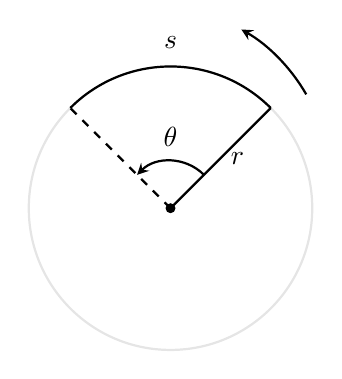
\begin{tikzpicture}[>=stealth, thick, scale=1.5]
        % 1. Draw the full circle in light gray
        \draw[gray!20] (0,0) circle (1.2cm);
        
        % 2. Draw the 90-degree "Pizza Slice" pointing up
        \coordinate (O) at (0,0);
        \draw (O) -- (45:1.2cm) node[midway, right] {$r$};
        \draw[dashed] (O) -- (135:1.2cm) node[midway, left]{};
        \draw[thick] (45:1.2cm) arc (45:135:1.2cm);
        
        % 3. Label for the arc 's'
        \node at (90:1.4cm) {$s$};
        
        % 4. Angle label theta inside
        \draw [->] (45:0.4cm) arc (45:135:0.4cm);
        \node at (90:0.6cm) {$\theta$};

        % 5. External rotation arrow
        \draw[->] (40:1.5cm) arc (30:60:1.5cm);
        
        % Origin point
        \fill (O) circle (1.2pt);
    \end{tikzpicture}
    & 
    % Wrap the table in a minipage aligned to the top [t]
    \begin{minipage}[t]{4cm}
        \vspace{-1cm} % Adjust this value to move the text up or down exactly where you want it
        \begin{tabular}{l}
            Circumference is $C = 2 \pi r$, \\
            the angle for a round trip on the \\
            circumference.
        \end{tabular}
    \end{minipage}
\end{tabular}
\]

\vspace{1em}

\[
\begin{tabular}{m{5cm} @{\hspace{1cm}} m{5cm}} % '@' adds specific spacing between columns
    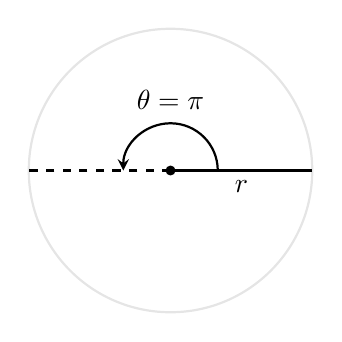
\begin{tikzpicture}[>=stealth, thick, scale=1.5]
    % 1. Draw the full circle in light gray
    \draw[gray!20] (0,0) circle (1.2cm);
    
    % 2. Define Center
    \coordinate (O) at (0,0);
    
    % 3. Draw the horizontal radius (Solid, to the right)
    % 0:1.2cm means 0 degrees (horizontal)
    \draw (O) -- (0:1.2cm) node[midway, below] {$r$};
    
    % 4. Draw the opposite radius (Dashed, to the left)
    % 180:1.2cm is the far left
    \draw[dashed] (O) -- (180:1.2cm);
    
    % 5. Draw the angle arrow (theta = pi)
    % It starts at 0 degrees and sweeps to 180 degrees
    \draw [->] (0.4,0) arc (0:180:0.4cm);
    \node at (90:0.6cm) {$\theta = \pi$};

    % Origin point
    \fill (O) circle (1.2pt);
\end{tikzpicture}
    & 
    % Wrap the table in a minipage aligned to the top [t]
    \begin{minipage}[t]{4cm}
        \vspace{-1cm} % Adjust this value to move the text up or down exactly where you want it
        \begin{tabular}{l}
            Arclength is $S = \pi r$, \\
            the area travelled along our arc.
        \end{tabular}
    \end{minipage}
\end{tabular}
\]

\[
\begin{tabular}{m{5cm} @{\hspace{1cm}} m{5cm}}
    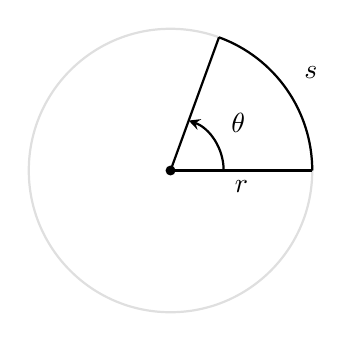
\begin{tikzpicture}[>=stealth, thick, scale=1.5]

        % Circle
        \draw[gray!25] (0,0) circle (1.2cm);

        % Center
        \coordinate (O) at (0,0);
        \fill (O) circle (1.2pt);

        % Radius lines
        \draw (O) -- (0:1.2cm) node[midway, below] {$r$};
        \draw (O) -- (70:1.2cm);

        % Arc corresponding to angle theta
        \draw[thick] (0:1.2cm) arc (0:70:1.2cm);

        % Arc label s
        \node at (35:1.45cm) {$s$};

        % Angle theta (radians)
        \draw[->] (0:0.45cm) arc (0:70:0.45cm);
        \node at (35:0.7cm) {$\theta$};

    \end{tikzpicture}
    &
    \begin{minipage}[t]{4cm}
        \vspace{-1cm}
        \begin{tabular}{l}
            Arclength is $S = \theta r$, the \\
            angle traveled in radians.
        \end{tabular}
    \end{minipage}
\end{tabular}
\]




\vspace{0.5em}

\subsection{Pendulum Continued}
What about the speed?
\begin{align*}
    \vec{v} = \dfrac{ds}{dt} = \dfrac{d}{dt}(r\theta)
\end{align*}

For circular motion, $r$ is constant so:
\begin{align*}
    \vec{v} = r\cdot\dfrac{d\theta}{dt}
\end{align*}

Finally, 
\begin{equation}
    a = \dfrac{d\vec{v}}{dt} = \dfrac{d}{dt} \left(r\dfrac{d\theta}{dt}\right) = r\dfrac{d^2 
    \theta}{dt^2}
\end{equation}

\vspace{1em}

Use Equation (4) in (3). For our pendulum, $r = L$.
\begin{align*}
    a_x = -g\sin\theta \\
    L\dfrac{d^2 
    \theta}{dt^2} = -g\sin\theta
\end{align*}

or

\begin{align*}
    \dfrac{d^2 \theta}{dt^2} = -\frac{g}{L}\sin\theta
\end{align*}

where $\theta$ is the angular position. Going back to our mass on a spring,
\begin{align*}
    \dfrac{d^2 x}{dt^2} = -\frac{k}{m}x
\end{align*}

\noindent where $x$ is the linear position of a mass on a spring. These are similar but not identical. We have $\sin\theta$ instead of $\theta$. We will consider the \textbf{small angle approximation.}

\subsubsection{Aside: Small Angle Approximation}














% =====================================================
% Copy this block for future lectures
% =====================================================
% \section{Lecture 2: Title Here}
%
% \subsection{Key Definitions}
%
% \subsection{Main Results}
%
% \subsection{Examples}
%
% \subsection{Remarks}

\end{document}
